\section{Distributed Ledger Technologies \& Blockchain}
Il problema del consenso è uno dei problemi fondamentali all'interno della blockchain.\\
Nell'ambito business è considerata, tra le tecnologie emergenti, una tecnologia essenziale.

\subsection{Storia}
La nascita della blockchain coincide con la nascita del progetto teorico del Bitcoin (2008). Gli algoritmi che stanno alla base di questa tecnologia invece erano già presenti nell'ambito dei sistemi distribuiti.\\
Nel 2009 esce una prima implementazione opensource di questo sistema. Da questo momento vengono sviluppate altre varianti. Questo meccanismo va bene non solo per denaro elettronico, ma ha potenziali applicazioni in molti altri ambiti. Potrebbe addirittura essere la base per avere applicazioni trusted distribuite, il cui output è trusted nonostante possano essere eseguite anche da nodi malevoli.
\\
Nel 2012-2013 vengono create altre criptovalute basate su DLT. 

\subsection{Perchè blockchain?}
La blockchain implementa un registro di cose che avvengono (ad esempio registro delle transazioni immobiliari/catasto) che è:
\begin{itemize}
    \item immutabile: posso andare a cercare indietro nella storia, ma non posso cancellare informazioni, posso solo aggiungerle
    \item distribuito: non si ha tutte le informazioni in uno stesso posto come un catasto o un registro centralizzato
    \item fault tolerant: non soltanto rispetto ad eventuali crash, ma anche rispetto a comportamenti bizantine, poiché non ho fiducia in alcun nodo che partecipa
\end{itemize}

\subsection{Il modello del sistema DLT}
È un sistema distribuito che ha le seguenti caratteristiche:
\begin{itemize}
    \item controllo decentralizzato, si ha quindi l'assenza di un nodo coordinatore
    \item i nodi sono gestiti da entità separate che non si fidano gli uni degli altri
    \item una copia dei record dei dati è salvata in ogni nodo
\end{itemize}
Il problema del consenso, in questo caso, è che i nodi devono essere d'accordo, non sull'ultimo dato memorizzato, bensì sulla storia dei dati. 

\subsection{Dati nella Blockchain}
Una blockchain è una sequenza storica di transazioni.\\
Una transazione è un record di dati (in ambito finanziario una transazione è un trasferimento di finanze ad esempio in BTC).


\subsection{Approccio}
Ogni transazione che viene inserita viene firmata (tramite criptazione asimmetrica, ossia utilizzando una chiave pubblica e una privata), e questa transazione firmata viene mandata (propagata) a tutti i nodi. \\
All'interno della blockchain si è identificati tramite la coppia chiave pubblica, chiave privata. Di queste coppie se ne possono avere diverse, quindi all'interno della blockhain si possono avere diverse identità(per questo è un sistema così anonimo).\\
Quando un nodo riceve una transazione deve validarla (in un ambiente finanziario un nodo potrebbe vedere nella sua storia se si hanno in fondi necessari per eseguire la transazione).\\
Le transazioni dopo che sono validate sono in stato pending siccome non sono ancora nella parte della catena.\\
\begin{center}
    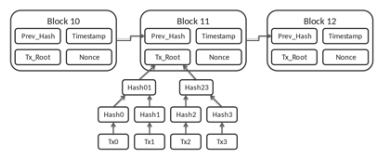
\includegraphics[width = .7\textwidth]{images/lezione6/approccio.png}
\end{center}
In una blockchain le transazioni sono raggruppate in blocchi (di n numeri di transazioni, dove n può essere diverso da un blocco a un altro) che hanno:
\begin{itemize}
    \item Timestamp di quando il blocco è stato creato
    \item Tx\_Root è una struttura dati (merkle tree: molto efficiente capire se una transazione è contenuta o meno nel blocco) che serve per memorizzare le transazioni che stanno dentro al blocco. Ogni transazione ha un hash che la rappresenta. 
    \item Nonce: un numero
    \item Prev\_Hash: collegamento al blocco precedente tramite il suo hash
\end{itemize}
\textit{Ogni nodo partecipante ha una copia della blockchain intera.}

\subsection{Problemi}
I sistemi di cui stiamo parlando sono asincroni, difficili da gestire a causa di latenza indecidibile, sincronizzazione imprecisa del clock e nodi malevoli, tutte caratteristiche che comportano:
\begin{itemize}
    \item l'ordine di arrivo delle transazioni possono essere diversi su diversi nodi
    \item alcune transazioni potrebbero contraddirsi a vicenda
    \item nodi diversi possono costruire diversi blocchi
    \item nodi diversi possono ritrovarsi con catene diverse (non si ha consenso)
\end{itemize}

\subsection{Consenso nella blockchain}
La sfida è quindi avere per ogni nodo il consenso sui blocchi e sulla sequenza di blocchi (sulla catena).\\
L'idea principale dell'algoritmo è:
\begin{enumerate}
    \item calcoliamo l'hash di ogni transazione e di un blocco
    \item quando calcolo l'hash del blocco inserisco nella funzione di hash anche l'hash del blocco precedente
    \item si include un trucco per rendere la computazione dell'hash del blocco molto dispendiosa(processo di mining), ma molto facilmente verificabile (proof of work)
    \item  se abbiamo un certo numero di nodi che vogliono fare un lavoro li si fanno competere e c'è una ricompensa (valuta di quella blockchain) per il vincitore, che si occuperà di distribuire il blocco calcolato a tutti gli altri nodi (è come eleggere un nodo che impone il suo blocco)
\end{enumerate}
L'hash di un blocco, di fatto, è la sua firma digitale. Modificando qualcosa all'interno della catena, la catena non sarà più valida, poiché occorrerà ri-validare tutti i blocchi che seguono attraverso il mining. \\
Per controllare se gli hash delle catene sono uguali, controllo l'hash dell'ultimo blocco di ciascuna catena: se sono uguali, ho il consenso sulla catena. Se non ho consenso ho il rischio che nodi diversi abbiano catene diverse.\\\\
Perchè viene dato un lavoro difficile al miner? \\
Perchè ci vorrà del tempo per risolverlo e quindi sarà più difficile avere soluzioni contemporanee. \\
Questo "puzzle" da risolvere viene calibrato in base alla quantità e alla capacità dei miner. Deve essere un problema risolvibile con algoritmi che operano con tecniche brute force, che si può far diventare più difficile progressivamente e che abbia una certa varianza.\\
Ma qual è questo problema così difficile da risolvere?

\subsection{Hashing}
Abbiamo una funzione di hash crittografica f (SHA-256):
\begin{itemize}
    \item dove f(A) ha una lunghezza fissa (per esempio 256 bit, indipendentemente dalla lunghezza dell'input A)
    \item che è resistente alle collisioni (se A diverso B anche f(A) diverso f(B)) 
    \item dove è molto difficile trovare A a partire da f(A)
    \item dove è molto facile calcolare f(A), cioè è facile verificare dati A e B se B = f(A)
\end{itemize}


\subsection{Algoritmo PoW nella Blockchain}
Il compito del miner è trovare il Nonce tale per cui il valore dell'hash finale sia più piccolo di un certo numero, scelto in modo collettivo, affinchè il tempo di risoluzione rimanga costante nel tempo.\\
Il computer deve provare con un meccanismo di brute force tutti i Nonce fino a quando non trova quello che soddisfa i requisiti.\\
È un problema progettato per richiedere un certo lasso di tempo, in modo da diminuire al minimo la probabilità che due miner risolvano l'enigma nello stesso momento.\\
Quando un miner risolve il puzzle lo annuncia a tutti.\\
Gli altri nodi, quando ricevono un messaggio da un nodo che dice di aver risolto un blocco, se effettivamente è stato verificato, lo aggiungono alla copia locale della loro catena. \\
\begin{center}
    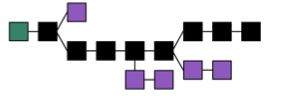
\includegraphics[width = .6\textwidth]{images/lezione6/chain.png}
\end{center}
La catena può avere dei branch (come possiamo vedere anche dalla foto), poiché siamo in una modalità concorrente, cioè i processi vengono eseguiti su nodi diversi ed è difficile prevedere chi finisce prima o dopo o quasi nello stesso momento. \\
È possibile che arrivino due blocchi entrambi validati e che abbiano lo stesso indirizzo del blocco precedente, nonostante siano diversi, formando quindi un branch.\\
La proprietà del Proof of Work fa si che ci sia una catena che si sviluppa più velocemente delle altre e che è quindi la porta ad essere la principale. \\
I blocchi che rimangono pendenti e che non fanno parte della catena prevalente, devono essere svuotati delle loro transazioni, che vengono rimesse nella pool di transazioni pending, a meno che non facciamo già parte di un blocco nella catena principale. \\
Saranno poi pescate in successivi tentativi di composizione dei blocchi.
(?) Un miner prende delle transazioni dal pool del pending, senza nessuna politica di selezione. Diversi miner possono prendere diverse transazioni. Se due miner sono al corrente di uno stesso blocco e sono d'accordo su di questo, prendono due insieme di transazioni diverse, lo risolvono e quando lo restituiscono al nodo vengono aggiunti entrambi generando il branch.(?)

\subsection{Proprietà della blockchain}
\begin{itemize}
    \item Assumendo che il maggior numero dei nodi stanno lavorando sulla stessa catena, quella che cresce più velocemente sarà la più lunga e la più veritiera.
    \item Un nodo malevolo se vuole modificare la transazione di un nodo intermedio deve anche ri-minare tutti i blocchi successivi e deve anche prevalere su tutti gli altri nodi della rete.
    \item Il meccanismo della blockchain è sicuro finchè più del 50\% del lavoro dei miner è onesto
\end{itemize}

\subsection{Limiti del Proof of Woork}
Ci sono tantissime critiche a questo algoritmo di consenso, per cui sono emerse altre proposte. \\
Non è il PoW che fa funzionare la blockchain, è l'algoritmo di consenso in generale ad essere importante.\\
I principali difetti sono:
\begin{itemize}
    \item consumo di energia e risorse (circa 1 miliardo di euro al giorno)
    \item numero di transazioni al secondo limitate
\end{itemize}

\subsection{Proof of Stake}
È detto proof-of-stake (PoS, vagamente traducibile in italiano come "prova che si ha un interesse in gioco") un tipo di protocollo per la messa in sicurezza di una rete di criptovaluta e per il conseguimento di un consenso distribuito. È basato sul principio che a ogni utente venga richiesto di dimostrare il possesso di un certo ammontare di criptovaluta. Si differenzia dai sistemi proof-of-work che sono basati su algoritmi di hash che validano le transazioni elettroniche. Peercoin è stata la prima criptovaluta ad introdurre sin dal lancio il sistema Proof of Stake senza mai implementarlo completamente. Altre note implementazioni del PoS sono BitShares, Nxt, BlackCoin e Cardano.

\subsubsection{Varianti per la selezione di un blocco}
Ogni qualvolta un nuovo blocco viene aggiunto alla blockchain, deve essere scelto il creatore del blocco successivo. Dato che quest'ultimo non può essere l'account che possiede la maggiore quantità della criptovaluta (altrimenti questo creerebbe tutti i blocchi), sono stati escogitati diversi metodi di selezione.


\paragraph{Selezione casuale (random)}
Nxt e BlackCoin utilizzano una funzione casuale per predire il generatore del blocco successivo, impiegando una formula che cerca il valore hash più basso rapportato alla dimensione della somma in gioco. Dato che la conoscenza delle somme è pubblica, ogni nodo della rete può predire - con ragionevole accuratezza - quale account si aggiudicherà il diritto di forgiare un nuovo blocco.

\paragraph{Selezione basata sull'anzianità}
La PoS di Peercoin mescola la selezione casuale con il concetto di "anzianità", un numero ottenuto tramite il prodotto del numero di monete per il numero di giorni in cui tali monete sono state possedute. Le monete che non sono state spese per almeno 30 giorni competono per la creazione del blocco successivo. Gli ammontari di monete più anziani e più grandi hanno una maggiore probabilità di firmare il blocco successivo. Eppure quando un ammontare di monete è utilizzato per firmare un blocco, questo ammontare deve ricominciare con "anzianità zero" e quindi aspettare almeno altri 30 giorni prima di poter firmare un altro blocco. E inoltre la probabilità di trovare il blocco successivo è massima dopo 90 giorni, per prevenire che somme consistenti e molto "anziane" possano dominare la blockchain. Questo processo mette in sicurezza la rete e produce gradualmente nuova valuta nel corso del tempo senza consumare una potenza computazionale significativa. Gli sviluppatori di Peercoin sostengono che questo renda più difficile attaccare la rete dato che cade il bisogno di piattaforme centralizzate di mining e inoltre acquistare più di metà delle monete è probabilmente più costoso che acquisire il 51\% della potenza di hashing della proof-of-work.

\paragraph{Selezione basata sulla velocità}
Il concetto di PoS di Reddcoin basata sulla velocità rivendica di incoraggiare la movimentazione di moneta piuttosto che il suo accumulo.

\paragraph{Selezione basata sul voto}
Invece di utilizzare solamente il concetto di posta in gioco (stake), i creatori dei blocchi possono essere selezionati mediante votazione. BitShares utilizza un sistema che comprende 101 delegati e sceglie casualmente tra essi.[1] Il voto della comunità aumenta l'incentivo dei creatori dei blocchi ad agire responsabilmente, ma al contempo apre alla prospettiva di scenari di sybil attack - come ad esempio nell'eventualità che un singolo utente impersoni i primi cinque delegati.

\subsection{Raft}
Raft è algoritmo per il consenso che è stato progettato per essere facile da capire. È l'equivante a Paxos a livello di fault-tolerance e performance.\\
Questo protocollo scompone il codice in sottoproblemi relativamente indipendenti tra loro e affronta ogni “pezzo” singolarmente.\\
Lo scopo principale di Raft è quello di rendere il consenso disponibile ad un pubblico sempre più vasto e che quest’ultimo sarà in grado di sviluppare nuovi sistemi basati sul consenso.\\
Raft si occupa della replica dei log. Intuitivamente, se si riesce a far apparire la stessa identica sequenza di log sulla maggior parte delle macchine, si è riusciti a far sì che quel cluster di macchine concordi su qualcosa.\\
In effetti, questo è chiamato trasmissione dell'ordine totale.\\ Se si riesce a far apparire ogni voce del log nella stessa posizione in un cluster di macchine, si può usarlo per implementare il consenso. \\
Ad esempio, se una macchina vuole proporre un valore e supponiamo che la sua ultima voce di registro sia nella posizione i, può provare a far sì che altre macchine mettano questo nuovo valore in i + 1 . Dopo che la maggior parte delle macchine nel cluster ha replicato quel valore in i + 1 , ora chiamiamo quel valore impegnato in i + 1 . Questo è effettivamente lo stesso che proporre un valore e farlo accettare da altri nei termini di Paxos.\\
Raft è un protocollo basato su leader. Nel suo normale corso operativo, un solo leader sarà eletto dal cluster di nodi. Gli altri nodi sono seguaci. Il leader accetta le richieste di scrittura del cliente e le replica ai follower.\\
Se si vogliono avere informazioni più approfondite su Raft si può leggere
\href{https://ichi.pro/it/protocollo-raft-consensus-reso-piu-semplice-160718622511489}{questo articolo} che ne spiega in dettaglio il funzionamento.


\subsection{Smart Contracts}
La blockchain è utile per salvare cose che vanno oltre a transazioni finanziarie. Ad esempio Ethereum è stata progettata per gli smart contracts.\\
Gli smart contract sono porzioni di codice software definiti come contratti self-executing.\\Sebbene originariamente sono stati proposti come versione digitale di contratti legali, possono essere dei programmi software generali.\\
Ogni contratto è salvato nella blockchain, diventando così immutabile.\\
Ogni nodo può verificare se le condizioni del contratto sono soddisfatte e eseguire determinate azioni (l'output deve essere validato in maniera distribuita). Alla fine tutti i nodi devono essere d'accordo sullo "stato" risultante.\\
Un esempio di applicazione potrebbe essere una piattaforma di crowdfounding senza autorità centrale.

\subsection{Permissionless vs Permissioned DLT}
Le blockchain di Bitcoin ed Ethereum sono chiamate permissionless poichè:
\begin{itemize}
    \item si ha un DL decentralizzato che traccia tutte le transazioni
    \item non ci sono terze parti fidate
    \item si ha accesso incondizionato al ledger
    \item si ha la validazione delle transazioni e la generazione di nuove monete da parte dei miners
    \item si ha la pseudo-anonimità dei partecipanti
    \item le transazioni sono immutabili
\end{itemize}
Esistono anche DLT permissioned, che vengono sfruttate soprattutto in ambito business dove ci sono molte istituzioni che usano questo meccanismo in un insieme trust limitato.\\
In queste DLT:
\begin{itemize}
    \item si ha un DL decentralizzato che traccia tutte le transazioni
    \item ci sono una o più terze parti fidate
    \item si ha un accesso condizionato al ledger
    \item  si ha la validazione delle transazioni e la generazione di nuove monete da parte dei miners
    \item si conosce l'identità dei partecipanti
    \item le transazioni sono immutabili
\end{itemize}

\subsubsection{Hyperledger Fabric}
Hyperledger nasce nel 2015 come consorzio di industrie che ha lo scopo di sviluppare una blockchain open-source per il business, hostata da Linux Foundation.\\
Fabric è uno dei sottoprogetti, originariamente gestito da IBM) che prevedeva:
\begin{itemize}
    \item permissioned DLT
    \item architettura modulare in grado di adattarsi a diversi requisiti: transazioni private, contratti confidenziali, diversi protocolli di consenso
    \item app (contratti) distribuite in linguaggi di programmazione generici
    \item nessuna dipendenza da criptovalute native
\end{itemize}



\begin{comment}
ociredeF


==============

ramO

Il problema del consenso è uno dei problemi fondamentali nel blockchain.
Nell'ambito business è considerata una tecnologia essenziale.
Nasce dalla nascita di bitcoin in avanti. Gli algoritmi che stanno alla base del paper che ha introdotto il bitcoin sono antecedenti. Il creatore di bitcoin lo ha ideato prendendo sputo da ricerca nei sistemi distribuiti. Questo whitepaper apparso nel 2008 è stato rivoluzionario. Firmato da uno pseudonimo, di cui ancora oggi non sappiamo il nome. 
Bitcoin: p2p cash system
Un mese prima dall'uscita del paper qualcuno ha registrato il nome Bitcoin, intuendo che avrebbe potuto rivoluzionre l'ambito finanziario.
Nel 2009 esce una prima implementazione di questo sistema open source. Da lì varie altre implementazioni e varianti. Questo meccanismo non va bene solo per denaro elettronico, ma ha potenziai applicazioni in molti altri ambiti. Potrebbe addirittura essere la base per avere applicazioni trusted distribuite, il cui output è trusted nonostante possano essere eseguite anche da nodi malevoli.

Nel 2013 nasce Ethereum e poi tante altre DLT.

La caratteristica di blockchain è che implementa un specie di registro delle cose che avvengono (ad esempio il registro delle transazioni immobiliari/catasto) che è immutabile (si può osservare tutta la storia). La novità è la distribuzione, non c'è un "catasto"/database(?) centralizzato che memorizza i dati, bensì è distribuito. L'obbiettivo è rendere storica l'informazione, immutabile (posso solo aggiungere e non posso cancellare), distribuita e fault tolerant (non soltanto crash, ma anche bizantine, poiché non ho fiducia in alcuni nodi che partecipano).

Le applicazioni della blockchain sono ampie. Dai quadri ai videogiochi, etc.

Il DLT System Model è un sistema distribuito. Ha un controllo decentralizzato, in cui ogni nodo esegue lo stesso codice e non c'è un controllore vero e proprio. Questi nodi sono gestiti da entità separate, non c'è un comune amministratore, e non si fidano gli uni degli altri (anche se ci sono DLT con assunzioni di trust). Dunque questo distribuito ha potenzialmente nodi con comportamento bizantino. Mettiamo una copia di tutto dappertutto. Tutti hanno una copia di questo "catasto".
Il problema del consenso, in questo caso, è che i nodi devono essere d'accordo, non sull'ultimo dato memorizzato, bensì sulla storia dei dati. 
Una blockchain è una sequenza storica di transazioni. Una transazione è un record di dati (in generale, dopodiché, essendo stata proposta in ambito finanziario ...).
Una transazione per convenzione deve avere stesso input e stesso output. Non si memorizza mai il saldo, bensì le entrate (?).

Ogni transazione che viene inserita viene firmata. Questa transazione firmata viene mandata a tutti i nodi della blockchain, perché la stessa informazione deve essere memorizzata da tutti. Nella blockchain si è identificati dalla coppia chiave pubblica/privata (se ne possono avere molte e quindi identità blockchain diverse). Quando un nodo riceve una transazione sa che arriva da un certo indirizzo blockchain. Nella transazione c'è anche la ciave pubblica del mittente in modo da fare verifiche ulteriori. C'è quindi un meccanismo di crittografia che garantisce l'origine.
Quando un nodo riceve la transazione, la valida. Come questo avviene fatto dipende dal tipo di applicazione. Bitcoin controlla dallo storico se aveva soldi dallo storico (?). Dopodiché la mette in un pool di transazioni pending. 
Da questo insieme di transazioni pending, si raggruppano in un blocco (non tutti i blocchi hanno stesso numero di transazioni). Questo blocco ha un timestamp (non necessariamente lo stesso di tutte le transazioni che sono dentro). Timestamp di quando ho fatto il blocco, non di quando ciascuna transazione è stata inserita.
ESEMPIO
Il blocco 11 contiene 4 tranazioni. Sono alla base dell'albero da Tx0 a Tx3. Sono organizzate in una struttura dati Merkle Tree, una struttura dati particolarmente efficiente per una determinata operazione. Queste transazioni hanno un corrispondente valore di hash. Abbiamo quindi una funzione di hash. Questa struttura dati è molto efficiente per capire se una transazione è contenuta oppure no nel blocco guardando l'hashing della radice. C'è inoltre un timestamp, un numero (nonce) e un "puntatore" contente un valore digitale che rappresenta il blocco precedente della catena. La cosa importante è che ognugno dei nodi ha un copia di questa blockchain. 
Blocchi e tranaszioni potrebbero avere timestamp diversi in diversi nodi, non avendo sincronizzazione perfetta. 
I problemi sono dovuti al fatto che i sistemi di cui stiamo parlando sono sistemi asincroni. Si possono fare assunzioni e accettare che qualcosa vada male, controllando poi che cosa va male. 
Problemi che in alcuni casi sono impossibili da risolvere in modo perfetto.
- La propagazione non arriva nello stesso ordine a tutti. 
- Transazioni possono essere contraddittorie
- Se le transazioni pending vengono accumulate da ogni nodo, posso avere che due nodi fanno blocchi diversi contemporaneamente.
- Possono avere catene diverse. Tutti devono avere stessa catena (problema del consenso).

L'idea dell'algoritmo proof of work è:
- calcoliamo l'hash di ciascun transazione, che da un valore come output che rappresenta quell'oggetto
- calcolo l'hash del blocco, inserendo nella funzione di hash del blocco l'identità del blocco precedente nella catena
- I nodi che calcolano l'ash del blocco devono fare un lavoro significativo (non tutti i nodi della blockchain lo fanno) chiamato mining. Alcuni dei nodi si rendono volontari di fare questo lavoro di calcolare l'hash secondo un certo trucco che è stato inserito. Chi guarda il lavoro fatto, immediatamente capisce se è fatto bene o male. Costoso da svolgere, ma immediatamente verificabile.
- Se abbiamo un certo numero di nodi (miner) che vogliono fare il lavoro, li facciamo competere. C'è un ricompensa in termini di valuta della blockchain. Si vuole eleggere quello che risolve per primo l'enigma matematico. Ci vuole anche un meccanismo per far sì che sia imrobabile (ma non impossibile) che due risolvano il problema nello stesso istante.
Diamo a ciascun miner un compito difficile in modo che ci debba mettere del tempo e sia molto improbabile che lo risolvano nello stesso momento. Questo puzzle viene calibrato man mano che i miner aumentano la capacità di risolvere il problema. 
Deve essere un problema risolvibile con brute force, che posso far diventare più difficile progressivamente e che abbia una certa varianza.

Abbiamo una funzione di hash crittografica (es. SHA256). Voglio che il suo output non sia dipendente dall'input in termini della lunghezza della stringa. Sempre stessa lunghezza. Se lo applico a due input diversi, l'output deve essere diverso. Deve essere molto difficile ricostruire input da output. Deve essere anche molto veloce calcolare l'hash e posso verificare facilmente che dato l'input A e l'output B, B = f(A).

Demo blockchain:
Il mining consiste nel trovare un nonce tale per cui l'hash del blocco sia più piccolo di un certo numero, scelto in modo collettivo affinché il tempo di risoluzione rimanga costante nel tempo. All'interno della blockchain, ogni blocco contiene l'hash del blocco precedente. L'hash di un blocco, di fatto, è la sua firma digitale. Modificando qualcosa all'interno della catena, la catena non sarà più valida, poiché occorrerà ri-validare tutti i blocchi che seguono attraverso il mining. Per controllare se gli hash delle catene sono uguali, controllo l'hash dell'ultimo blocco di ciascuna catena. Se sono uguali, ho il consenso sulla catena. Se non ho consenso, ho il rischio che nodi diversi abbiano catene diverse (?).

Il numero di transazioni può essere diverso nei diversi blocchi.

I messaggi sono firmati, per cui diventa più semplice risolvere il problema di consenso bizantino. Devo avere almeno la maggioranza dei nodi che non hanno il comportamento bizantino (2k + 1) per falsificare la transazione (?).

Risultato rilevante è il trucchetto della PoW. Quando un miner risolve il puzzle, lo annuncia a tutti. Gli altri nodi, quando ricevono un messaggio che dice di aver risolto un blocco (viene quindi mandato blocco e hash che dimostra la risoluzione facilmente verificabile), se effettivamente è stato verificato, lo aggiunge alla copia locale della catena. La catena può avere dei branch, poiché siamo in una modalità concorrente, cioè i processi vengono eseguiti su nodi diversi ed è difficile prevedere chi finisce prima o dopo o quasi nello stesso momento. è possibile che arrivino due blocchi entrambi validati e che abbiano lo stesso indirizzo del blocco precedente, nonostante siano diversi, formando quindi un branch. La proprietà del PoW fa si che ci sia una catena che si sviluppa più velocemente delle altre e che è quindi quella condivisa da tutti. I blocchi che rimangono pendenti e che non fanno parte della catena prevalente, deve rimettere le transazioni che erano in questo blocco nella pool di pending, a meno che non facciamo già parte di un blocco nella catena. Saranno pescate in successivi tentativi di composizione dei blocchi.

Un miner prende delle transazioni dal pool del pending, però non c'è una politica di selezione. Diversi miner possono prendere diverse transazioni. Se due miner sono al corrente di uno stesso blocco e sono d'accordo su di questo, prendono due insieme di transazioni diverse, lo risolvono e quando lo restituiscono al nodo vengono aggiunti entrambi generando il branch.

I miner sono anche nodi della catena.

Le proprietà che emergono sono:
- se la maggior parte dei nodi lavorano sulla stessa catena ...
- non solo, se vuole cambiare qualcosa nella catena, deve ricalcolare i blocchi, ma deve anche imporsi sulla catena più lunga (?).
- più del 50\% del lavoro dei miner deve essere onesto

Ci sono tantissime critiche a questo algoritmo di consenso, per cui sono emerse altre proposte. Non è il PoW che fa funzionare la blockchain, è l'algoritmo di consenso in generale ad essere importante.

L'elettricità costa parecchio per fare PoW (1 miliardo al giorno) e le transazioni sono poche.

Il consenso non c'è mai sull'ultimo blocco soltanto, ma dev'essere sulla storia della catena.

Sono stati proposti diversi algoritmi di consenso, ad esempio Raft, algoritmo di consenso per altro tipo di blockchain: permissioned (?).
Proof of stake sostiene che chi ha più potere/risorse decide quale blocco aggiungere. In più c'è un meccanismo randomico, non c'è la selezione esatta di chi ha più risorse. Inoltre c'è il discorso dell'età: da quanto tempo questo verificatore del blocco fa parte della blockchain? Più è alto è il tempo, più è alta la fiducia. L'intuizione dietro a questa scelta è che il danno che loro avrebbero nell'essere malevoli nella blockchain è superiore al guadagno. Quando uno di questi volontari viene scelto, il suo account viene congelato fino a quando non si capisce che la validazione è stata corretta e dopodiché viene rilasciato.

In Raft viene fatta un'elezione in modo distribuito. Non sempre è l'id maggiore che vince, poiché questo può essere costruito per esempio guardando quanti soldi hanno nel conto e far emergere quello che ha più soldi. Bisogna escludere quello dal comportamento malevolo, poiché si è deciso di farlo in termini di fiducia. Se il validatore cerca di compromettere il sistema/validare transazioni fraudolenti dentro al blocco, perdono tutto.

Come si previene il double spending problem? (uso i miei soldi per due transazioni cercando di comprare due cose con gli stessi soldi)
VIDEO

Nel 2012-13 è apparso un articolo che propone una generalizzazione dell'uso di blockchain, rendendo esplicita la cosa. Da qui nasce Ethereum, che generalizza, rispetto a transazioni finanziarie, a smart contract (più eterogenea) e ha un suo linguaggio per scrivere gli smart contract.

Queste blockchain vengono chiamate permissionless: chiunque può decidere di partecipare e vedere le transazioni dentro la blockchain. C'è pseudoanonimità dei partecipanti. 

Ci sono anche DLT permissioned. Soprattutto in ambito business ci sono molte istituzioni che usano questo meccanismo tra un insieme di aziende (trust limitato). Limitare la partecipazione e aggiungere un controllo. Abbiamo identità nota dei partecipati. Ci sono delle identità trusted. Ci sono anche qui criptovalute legate a questo. Una di queste piattaforme per la generazione di DLT è hyperledger, in particolare hyperledger fabric (inizialmente fatto da IBM e poi ceduto). È possibile sviluppare gli smart contract (in ethereum c'è un linguaggio apposta) con general purpose programming languages, posso quindi scrivere codice all'interno dei dati che vengono racchiusi in blocchi.

------------
Fabbio
DLT: tecnologie blockchain

Nell'ambito business la blockchain è considerata una tecnologia essenziale. 
Storia:
Nel 2008 nasce un paper firmato da satoshi nakamoto (pseudonimo) intitolato Bitcoin. Bitcoin è un peer-to-peer cash system. Il mese prima dall'uscita del paper qualcuno aveva registrato il nome Bitcoin.
Nel 2009 esce la prima implementazione opensource e da lì in poi varie implementazioni e varianti.
Il meccanismo ha potenziali applicazioni in moltissimi ambiti. Potrebbe essere la base per avere applicazioni distribuite trusted il cui output è trusted nonostante possano essere eseguite anche da nodi malevoli.

nel 2013 esce ETH e via...

La caratteristica di blockchain che ispira altre applicazioni oltre al denaro elettronico è che implementa un registro delle cose che avvengono (tipo registro transazioni immobiliari o catasto immobiliare..). 
A differenza dei database il "catasto" viene distribuito su vari nodi. L'obiettivo è rendere storica, immutabile e full tolerance l'informazione.


Il modello del sistema DLT
-E' un sistema distribuito
-Ha un controllo decentralizzato in cui non c'è un coordinatore e ogni nodo esegue lo stesso codice
-I nodi sono gestiti da entità separate e non si fidano gli uni degli altri
Dunque il sistema distribuito ha assumibilmente nodi con comportamento "bizzantino"

Problema del consenso:
I nodi devono essere d'accordo su di uno storico dei dati. I nodi devono essere d'accordo sulla storia dei dati.

DATI NELLA BLOCKCHAIN
Una blockchain è una sequenza storica di transazioni
Transazione: Record di dati. Nell'ambito finanziario [A trasferisce x a B]
Una transazione per convenzione deve avere lo stesso input e lo stesso output.

L'APPROCCIO BLOCKCHAIN
Ogni transazione inserita viene firmata. Si utilizza il meccanismo di chiavi asimmetriche e ogni partecipante ha una chiave privata e una pubblica. Quando una transazione viene firmata, questa viene mandata a tutti i nodi della blockchain.
Quando un nodo riceve una transazione sa da quale nodo arriva. 
Nel codice condiviso che tutti i nodi hanno, c'è una porzione che dice "Quando arriva una transazione validala". Dunque il nodo che riceve va a vedere nello storico se la transazione è plausibile. 
Dunque: A mette una tranazione nel sistema che va a tutti i nodi. Chi la riceve guarda nello storico se è valida. Poi la mette in un pool di transazioni pending.
QUANDO PASSA IN UNO STATO APPROVED?

APPROCCIO BLOCKCHAIN:
Dall'insieme di transazioni pending, si raggruppano in un blocco (non tutti i blocchi hanno lo stesso numero di transazioni), il blocco ha un timestamp che non è lo stesso di tutte le transazioni che ha al suo interno. Nel blocco X (11 nelle slide) c'è il TX room: struttura dati per memorizzare le transazioni nel blocco. Ogni transazione ha il corrispondente valore di hash e la struttura dati ha la particolarità che è molto efficiente capire se una transazione è avvenuta o no.
C'è un certro numero di transazioni nel blocco e c'è una funzione per capire molto velocemente se all'interno del blocco c'è o meno la transazioni.
Da un blocco all'altro si collegano tramite un puntatore (valore digitale del blocco precedente viene scritto nel blocco successivo e viceversa). 
Ognuno dei nodi ha la copia di questa blockchain.

PROBLEMI:
I blocchi e le transazioni potrebbero avere timestamp diversi su diversi nodi. 
I problemi sono dovuti al fatto che i sistemi sono asincroni dove possono capitare le cose più bizzarre. Alcune transazioni potrebbero essere contraddittorie. Nodi diversi potrebbero creare blocchi diversi. Tutti i nodi devono avere la stessa blockchain. (Problema del consenso)

CONSENSO DELLA BLOCKCHAIN
Idea: si calcola l'hash di ogni transazione che da in output un certo valore che rappresenta l'oggetto. Calcolo l'hash del blocco. Quando calcolo l'hash del blocco inserisco l'identità digitale del blocco precedente e ci includo...
Non tutti i nodi della blockchain fanno il lavoro del calcolo dell'hash, e questo lavoro viene fatto dai miners. I miners introducono nella blockchain nuova valuta.
Alcuni dei nodi dunque si rendono volontari per calcolare l'hash con un trucco particolare. Il lavoro è duro e costoso ma immediatamente verificabile. (Idea dietro l'algoritmo di consenso)
Se si hanno un certo numero di nodi che vogliono minare, li si fa competere su di un blocco. C'è un compenso nella valuta della blockchain. Diversi nodi dunque si mettono a validare un blocco è tra tutti questi bisogna sceglierne uno. Quello che si elegge è quello che risolve prima "l'enigma matematico". Ci può essere il caso in cui 2 riescono risolvere il puzzle allo stesso momento.

PROBLEMI DIFFICILI:
perchè deve essere difficile? Perchè devono metterci tempo così che tutti finiscano in tempi differenti. La difficoltà del puzzle viene aumentata in base alla capacità del miner di risolvere il problema. Il problema deve essere un problema che dal punto di vista computazionale viene risolto in bruteforce, può avere una certa varianza (puoi essere fortunato o sfortunato a risolverlo).
Statisticamente è più difficile che più miners lo risolvono a diversi istanti.

QUAL è QUESTO PROBLEMA?
Funzione di Hashing crittografica con proprietà tipo:
Output indipendente dalla lunghezza dell'input.
Deve essere collision resistent.
Dallì'output deve essere quasi impossibile risalire all'input.
Deve essere facile da verificare.

PROPRIETA' BLOCKCHAIN:
La catena che cresce più velocemente sarà quella che merita fiducia. 


\end{comment}